\documentclass{article}[a4paper, oneside, 11pt]
\usepackage[T1]{fontenc}
\usepackage[utf8]{inputenc}
\usepackage{calc}
\usepackage{amsmath, amssymb, amsthm, thmtools, amsfonts}
\usepackage{mathtools}
\usepackage[nochapters,pdfspacing]{classicthesis}
%\usepackage{hyperref}% clashes with classicthesis
\usepackage{cleveref}
\usepackage[siunitx]{circuitikz}
\usepackage{booktabs}
\usepackage{graphicx}
\usepackage{caption}
\usepackage{geometry}
\usepackage{float}
\usepackage{mdframed}
\usepackage{xcolor}
\usepackage{siunitx}
\usepackage[italian]{babel}
\usepackage{pgfplots}
\usepackage{titling}
\usepackage{listings}
\usepackage{lmodern}
\usepackage{url}
\usepgfplotslibrary{external} 
\tikzexternalize

\pgfplotsset{compat=1.15}
\lstset{
language=Python,
basicstyle=\ttfamily,
columns=fullflexible,
keepspaces=true,
}
\mdfsetup{linewidth=0.6pt}
\graphicspath{{./figs/}}
\makeatletter
\def\input@path{{./figs/}}
%or: \def\input@path{{/path/to/folder/}{/path/to/other/folder/}}
\makeatother

\newcommand{\eps}{\varepsilon}
\renewcommand{\phi}{\varphi}
\newcommand{\loc}{\mathit{loc}}
\newcommand{\weakto}{\rightharpoonup}
\newcommand{\implied}{\Longleftarrow}
\let\subsetstrict\subset
\renewcommand{\subset}{\subseteq}
\renewcommand{\supset}{\supseteq}

% calligraphic letters
\newcommand{\A}{\mathcal A}
\newcommand{\B}{\mathcal B}
\newcommand{\C}{\mathcal C}
\newcommand{\D}{\mathcal D}
\newcommand{\E}{\mathcal E}
\newcommand{\F}{\mathcal F}
\newcommand{\FL}{\mathcal F\!\mathcal L}
\renewcommand{\H}{\mathcal H}
\newcommand{\K}{\mathcal K}
\renewcommand{\L}{\mathcal L}
\newcommand{\M}{\mathcal M}
\renewcommand{\P}{\mathcal P}
\renewcommand{\S}{\mathcal S}
\newcommand{\U}{\mathcal U} %% intorni

% blackboard letters
\newcommand{\CC}{\mathbb C}
\newcommand{\HH}{\mathbb H}
\newcommand{\KK}{\mathbb K}
\newcommand{\NN}{\mathbb N}
\newcommand{\QQ}{\mathbb Q}
\newcommand{\RR}{\mathbb R}
\newcommand{\TT}{\mathbb T}
\newcommand{\ZZ}{\mathbb Z}

%\newcommand{\abs}[1]{{\left|#1\right|}}
\newcommand{\Abs}[1]{{\left\Vert #1\right\Vert}}
\newcommand{\enclose}[1]{{\left( #1 \right)}}
\newcommand{\Enclose}[1]{{\left[ #1 \right]}}
\newcommand{\floor}[1]{\left\lfloor #1 \right\rfloor}
\newcommand{\ceil}[1]{\left\lceil #1 \right\rceil}

\newcommand{\To}{\rightrightarrows}
\renewcommand{\vec}[1]{\boldsymbol #1}
\newcommand{\defeq}{:=}
\DeclareMathOperator{\divergence}{div}
\renewcommand{\div}{\divergence}
\DeclareMathOperator{\Imaginarypart}{Im}
\renewcommand{\Im}{\Imaginarypart}
\DeclareMathOperator{\Realpart}{Re}
\renewcommand{\Re}{\Realpart}
%\DeclareMathOperator{\arg}{arg}
\DeclareMathOperator{\tg}{tg}
\DeclareMathOperator{\arctg}{arctg}
\DeclareMathOperator{\settsinh}{settsinh}
\DeclareMathOperator{\settcosh}{settcosh}
\DeclareMathOperator{\tr}{tr}
\DeclareMathOperator{\im}{im}
\DeclareMathOperator{\sgn}{sgn}
\DeclareMathOperator{\diag}{diag}

\declaretheoremstyle[
spaceabove=6pt, spacebelow=6pt,
headfont=\normalfont\bfseries\itshape,
notefont=\mdseries, notebraces={(}{)},
bodyfont=\normalfont,
postheadspace=1em,
qed=,
%shaded={rulecolor=pink!30,rulewidth=1pt,bgcolor=pink!10}
]{exercise_style}

\declaretheoremstyle[
spaceabove=6pt, spacebelow=6pt,
postheadspace=1em,
qed=,
%shaded={rulecolor=blue!20,rulewidth=1pt,bgcolor=blue!5}
]{theorem_style}

\declaretheoremstyle[
spaceabove=6pt, spacebelow=6pt,
postheadspace=1em,
qed=,
%shaded={rulecolor=yellow!50,rulewidth=1pt,bgcolor=yellow!5}
]{axiom_style}

\declaretheorem[name=Teorema]{theorem}
\declaretheorem[name=Lemma,sibling=theorem]{lemma}
\declaretheorem[name=Proposizione,sibling=theorem]{proposition}
\declaretheorem[name=Corollario,sibling=theorem]{corollary}
\declaretheorem[name=Paradosso,sibling=theorem]{paradox}
\declaretheorem[style=axiom_style,name=Assioma,sibling=theorem]{axiom}
\declaretheorem[name=Definizione,sibling=theorem]{definition}
\declaretheorem[style=exercise_style,name=Esempio,sibling=theorem]{example}
\declaretheorem[style=exercise_style,name=Esercizio,sibling=theorem]{exercise}
\declaretheorem[style=exercise_style,name=Osservazione,sibling=theorem]{remark}

% Logarithm with arbitrary base.
% -> log_10
\newcommand{\llog}[1][10]{\log_{#1}}

% Absolute value.
% -> |x|
\newcommand{\abs}[1]{\left| #1 \right|}

% Powers.
% -> x^a
\newcommand{\power}[2][2]{\left( #2 \right)^{#1}}

% Square.
% -> x^2
\newcommand{\sq}[1]{\power[2]{#1}}

% Expansion of the binomial coefficient.
% -> n1!/(n2!(n1 - n2)!)
\newcommand{\binomexpr}[2]{\frac{#1!}{#2!(#1 - #2)!}}

% Expression evaluation at a given point with square brackets.
% -> [x]_{a}
\newcommand{\at}[2]{\left[ #1\right]_{\makebox[-1pt][l]{${\scriptstyle#2}$}}}

% Expression evaluation in an interval.
% -> [x] _{a}^{b}
\newcommand{\eval}[3]{\left.#1%
  \right|_{\makebox[-1pt][l]{${\scriptstyle#2}$}}^{\makebox[-1pt][l]{${\scriptstyle#3}$}}}

% Upright d in math mode (for differentials).
% -> d
\newcommand{\ud}{\mathrm{d}}

% Differential.
% -> dx
\newcommand{\diff}[1][x]{\,\ud{#1}}

% Base command for defining derivatives.
% -> df/dx or d^kf/dx^k
\newcommand{\basederivative}[4][]{%
  \displaystyle%
  \ifx\\#1\\\frac{#4#2}{#4#3}%
  \else%
  \frac{#4^#1#2}{#4#3^#1}%
  \fi%
}

% Total derivative.
% -> df/dx(x) or d^kf/dx^k(x)
\newcommand{\td}[4][]{%
  \basederivative[#1]{#2}{#3}{\ud}%
  \ifx\\#4\\%
  \else%
  \mkern-4mu\left(#4\right)%
  \fi%
}

% Partial derivative.
% -> df/dx(x) or d^kf/dx^k(x)
\newcommand{\pd}[4][]{%
  \basederivative[#1]{#2}{#3}{\partial}%
  \ifx\\#4\\%
  \else%
  \mkern-4mu\left(#4\right)%
  \fi%
}

\newcommand{\intinf}{\int_{-\infty}^{\infty}\!\!\!}

\newcommand{\cinterval}[2]{\left[\, #1,~#2 \,\right]}

\newcommand{\linterval}[2]{\left[\, #1,~#2 \,\right)}

\newcommand{\rinterval}[2]{\left(\, #1,~#2 \,\right]}

\newcommand{\ointerval}[2]{\left(\, #1,~#2 \,\right)}

\newcommand{\prob}[1]{\displaystyle P\left(#1\right)}

\newcommand{\pvalue}{\emph{$p$-value}}

\newcommand{\cond}{\,|\,}

\newcommand{\expect}[1]{\displaystyle E\left[#1\right]}

\newcommand{\mom}[2][]{\displaystyle {\cal M}_{#2}\ifx\\#1\\\else(#1)\fi}

\newcommand{\momalg}[1]{\displaystyle \lambda_{#1}}

\newcommand{\momcen}[1]{\displaystyle \mu_{#1}}

\newcommand{\skewness}{\displaystyle \gamma_1}

\newcommand{\kurtosis}{\displaystyle \gamma_2}

\newcommand{\charf}[1][x]{\phi_{#1}}

\newcommand{\momgenf}[1][x]{M_{#1}}

\newcommand{\fwhm}{{\scriptstyle \textsc{FWHM}}}

\newcommand{\hwhm}{{\scriptstyle \textsc{HWHM}}}

\newcommand{\median}{\mu_{\nicefrac{1}{2}}}

\newcommand{\var}[1]{\ensuremath{\text{Var}\left(#1\right)}}

\newcommand{\cov}[2]{\ensuremath{\text{Cov}\left(#1, #2\right)}}

\newcommand{\corr}[2]{\ensuremath{\text{Corr}\left(#1, #2\right)}}

\newcommand{\like}{\mathcal L}

\newcommand{\likelihood}[2][]{\like\ifx\\#2\\\else(#2\ifx\\#1\\\else;#1\fi)\fi}

\newcommand{\chisq}{\ensuremath{\chi^2}}

\newcommand{\chisquare}[2][]{\chisq\ifx\\#2\\\else(#2\ifx\\#1\\\else;#1\fi)\fi}

\newcommand{\loglikelihood}[2][]{\log\likelihood[#1]{#2}}

\newcommand{\pdf}[3][]{#2(#3\ifx\\#1\\\else;#1\fi)}

\newcommand{\binomialpdf}[2][]{\pdf[#1]{\mathcal B}{#2}}

\newcommand{\multinomialpdf}[2][]{\pdf[#1]{\mathcal M}{#2}}

\newcommand{\poissonpdf}[2][]{\pdf[#1]{\mathcal P}{#2}}

\newcommand{\uniformpdf}[2][]{\pdf[#1]{u}{#2}}

\newcommand{\exponentialpdf}[2][]{\pdf[#1]{\varepsilon}{#2}}

\newcommand{\gausspdf}[2][]{\pdf[#1]{N}{#2}}

\newcommand{\chisquarepdf}[2][]{\pdf[#1]{\wp}{#2}}

\newcommand{\cauchypdf}[2][]{\pdf[#1]{c}{#2}}

\newcommand{\erf}[1]{\ensuremath{\text{erf}\left(#1\right)}}

\newcommand{\dccases}[4][]{#2 \ifx\\#2\\\else=\fi %
  \begin{cases}
    \displaystyle #3 & \text{per variabili discrete}\\
    \displaystyle #4 & \text{per variabili continue}#1
  \end{cases}
}
\newcommand\Scaleforall[1]{\vcenter{\hbox{\scalefont{#1}$\forall$}}}

\DeclareMathOperator*\forevery{%
  \vphantom\sum
  \mathchoice{\Scaleforall{2}}{\Scaleforall{1.4}}{\Scaleforall{1}}{\Scaleforall{0.75}}}
 
 % Default fixed font does not support bold face
\DeclareFixedFont{\ttb}{T1}{txtt}{bx}{n}{12} % for bold
\DeclareFixedFont{\ttm}{T1}{txtt}{m}{n}{12}  % for normal

% Custom colors
\usepackage{color}
\definecolor{deepblue}{rgb}{0,0,0.5}
\definecolor{deepred}{rgb}{0.6,0,0}
\definecolor{deepgreen}{rgb}{0,0.5,0}

\geometry{a4paper, left=25mm, right=25mm, top=30mm, bottom=30mm}
\title{Modellizzazione della resistenza di diodi a giunzione PN per alte correnti di lavoro}
\author{L.~Ciucci(\thanks{Dipartimento di Fisica E.~Fermi, Universit\`a di Pisa - Pisa, Italy} )~\and S.~Bruzzesi(\protect\footnotemark[1] )~\and M.~Romagnoli(\protect\footnotemark[1] )~\and M.~Alighieri(\protect\footnotemark[1] )~\and B.~Tomelleri(\protect\footnotemark[1] )}
\date{2020/11/01}

\begin{document}
\maketitle

%================================================================
%                            Riassunto
%================================================================
\begin{mdframed}
\textbf{Riassunto:} --- Studiamo il comportamento di diodi in silicio PN,
esplorando la propria curva caratteristica $V - I$ al di fuori dei regimi di
lavoro ordinari, tramite campionamenti digitali dei segnali ai capi del
componente. Discutiamo la presenza di una componente resistiva del diodo e ne
misuriamo l'entità, al fine di arrivare ad un modello teorico in grado
giustificare eventuali deviazioni dal modello di Shockley, verso una risposta
-ohmica- dovuta alla resistenza della giunzione PN al passaggio di correnti.\\\\
PACS 01.40.-d – Education.\\
PACS 01.50.Pa – Laboratory experiments and apparatus.
\end{mdframed}


%================================================================
%                         Introduzione
%================================================================
\section{Introduzione}
L'alta resistività intrinseca al silicio, di cui è composta la giunzione
bipolare, comporta la presenza di una sua componente resistiva: questa 
risulta sempre meno trascurabile agli effetti del passaggio di corrente
attraverso il diodo, all'aumentare della tensione ai suoi capi e della sua 
temperatura. Per poter modellare la componente -ohmica- di un diodo
percorso da correnti alte si propone un modello semplice di resistenza
parassita in serie, in grado di descriverne gli effetti, verificandone 
sperimentalmente la validità.


%================================================================
%                         Cenni teorici
%================================================================
\section{Cenni Teorici}
Secondo le ipotesi, un diodo reale può essere schematizzato quale un resistore ohmico ed un diodo ideale in serie. Pertanto ci aspettiamo che la corrente che attraversa tali elementi sia la medesima:
\begin{equation}
I = \frac{\Delta V_{resistore}}{R} = I_0 ( e^{\frac{\Delta V_{diodo}}{\eta V_t}} - 1)
\end{equation}
dunque la relazione che lega la corrente e la tensione ai capi del diodo può essere espressa secondo la legge:
\begin{equation}\label{eq: model}
\Delta V = \Delta V_d + \Delta V_r = \eta V_T  \ln{\frac{I+I_0}{I_0}} + RI
\end{equation}
(inserire una figura per far capire cosa sono I e $\Delta V$)\newline
(inserire dei grafici di confronto)


%================================================================
%                Metodo e apparato sperimentale
%================================================================
\section{Metodo e apparato sperimentale}
Il circuito sotto studio lavora con correnti relativamente alte, per evitare sostanziali aumenti di temperatura nei componenti ed eventuali danni agli stessi si imprimono correnti impulsate.
La durata degli impulsi è di circa 150 $\mu$s (da misurare meglio) che corrisponde ad un'energia impressa inferiore a 1 mJ dunque ad un aumento della temperatura del semiconduttore inferiore a 0.5 K.
%Dovendo lavorare con correnti relativamente alte per il circuito sotto studio,
%al fine di minimizzare effetti termici-dissipativi secondari ed evitare danni
%all'apparato, si imprimono sui componenti correnti pulsate o di durate molto
%brevi, limitando dunque il trasferimento di energia sui componenti.

%================================
%           Apparato
%================================
\subsection{Apparato}
L'apparato sperimantale è costituito da un circuito, realizzato su basetta sperimentale, il cui scopo è generare correnti impulsate attraverso il diodo D1 e la resistenza R1. La misura della differenza di tensione ai capi di questa permette stima della corrente che attraversa il diodo, per esplorare ampie zone di lavoro del diodo è stata cambiata opportunamente scegliendo tra le seguenti resistenze:\newline
TABELLA\newline
Nel circuito può essere individuata una parte che si ocupa della carica e scarica controllata del condensatore C1, il cui scopo è quello di fornire una tensione che possa essere facilmente regolata e sufficientemente stabile durante un impulso. Un'altra parte del circuito si occupa di collegare a comando il condensatore alla serie R1-D1 attraverso un MOS-FET.\newline
Il circuito è alimentato da 2 tensioni fornite da un alimentatore stabilizzato switching e da un Buck Boost Converter, un segnale fornito su T2 provoca la carica del condensatore mentre su T3 la sua scarica. Un segnale (invertito) su T1 innesca l'impulso di corrente sul diodo.\newline
La tensione di C1 è misurata attraverso un partitore di tensione collegato ad OUT3 ed alla scheda di controllo mentre la tenisone ai punti OUT1 e OUT2 è letta direttamente.\newline
Come MCU per la gestione dell'apparato è stata scelta la scheda \verb+Teensy 3.2+\cite{teensy}, questa si occupa del controllo dei segnali e delle letture analogiche. In particolare Teensy permette la lettura analogica sincronizzata differenziale veloce, essendo dotato di due ADC, entrambi con una risoluzione reale di 12 bit. La lettura differenziale è fondamentale per acquisire coppie di dati per le tensioni ai capi del diodo e della resistenza.\newline

\begin{figure}[!htb]
	\centering 
 		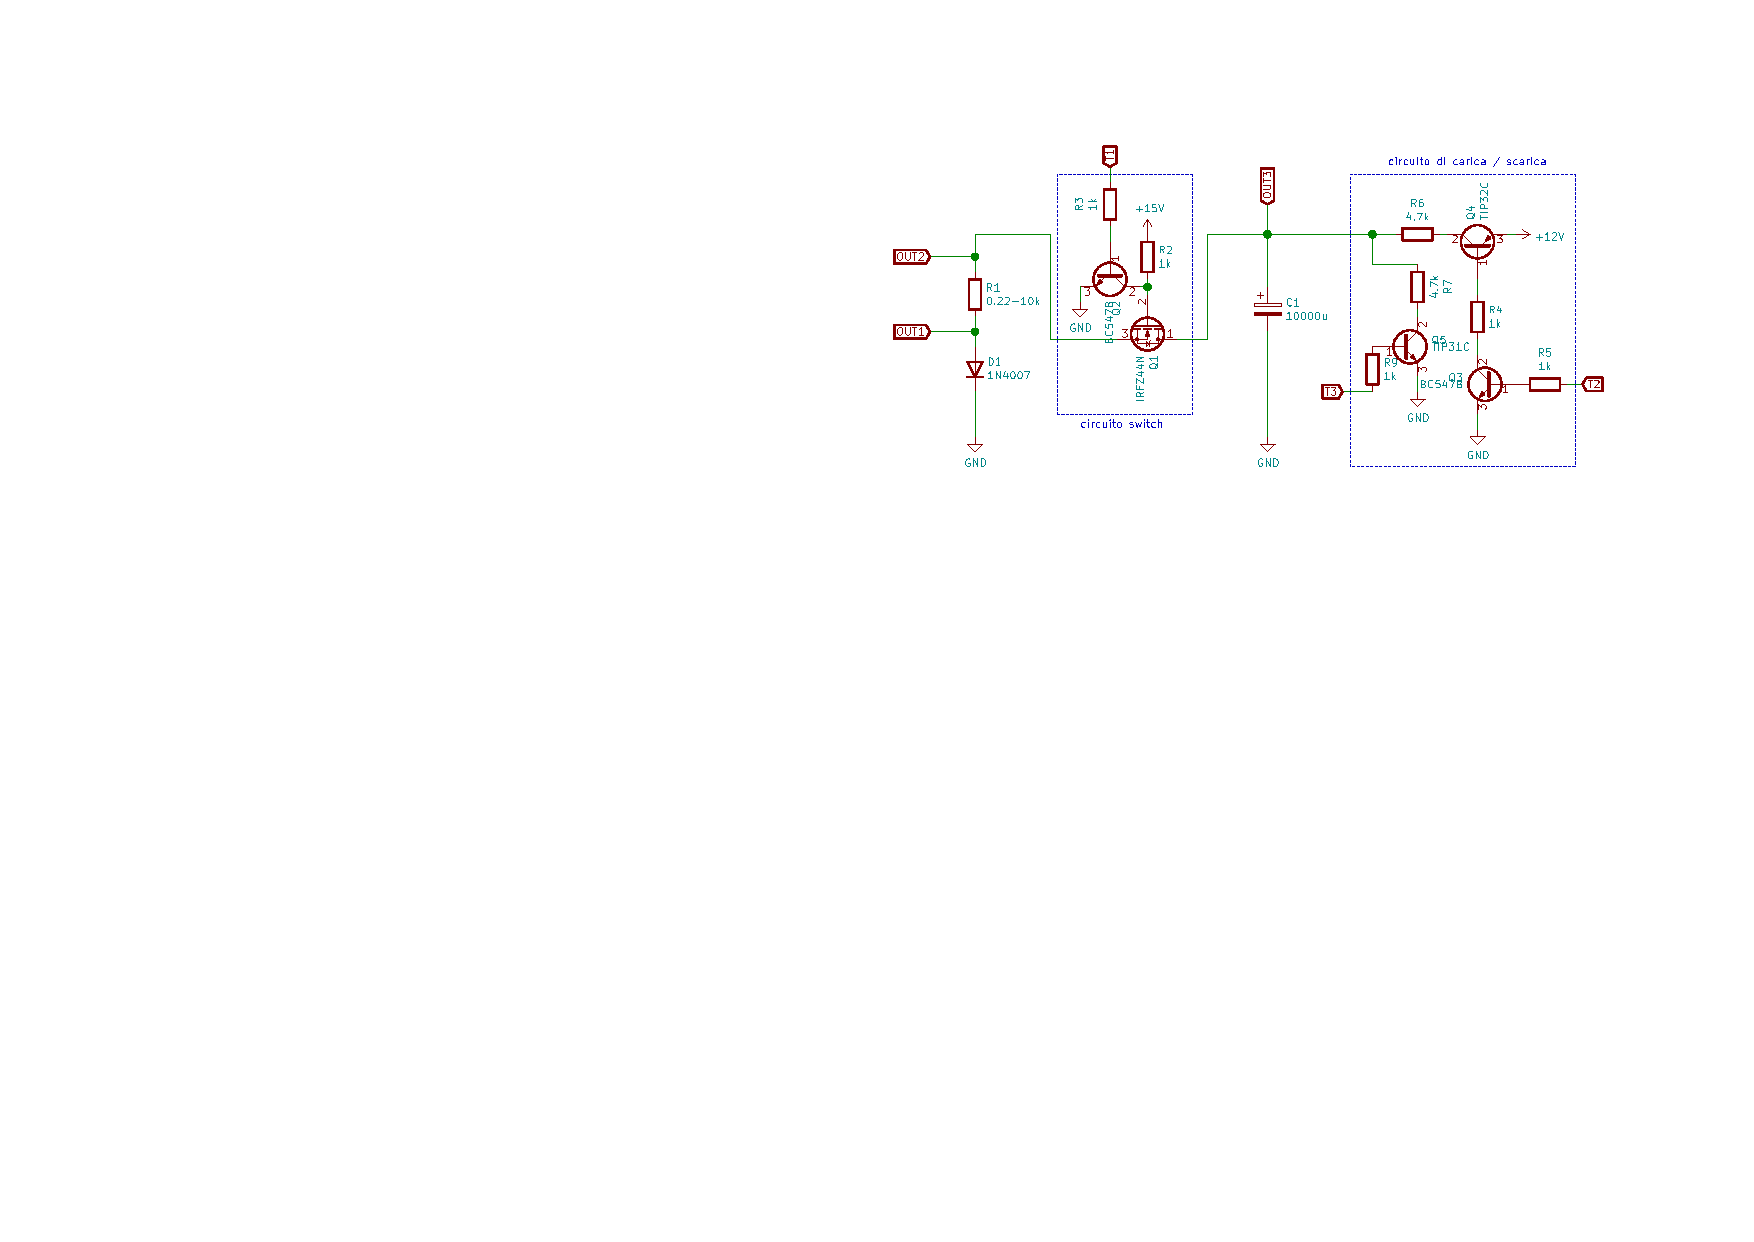
\includegraphics[scale=1.3]{./gestione.pdf}
 	\caption{Circuito globale per la gestione del diodo \label{sch:gest}}
\end{figure}
\begin{figure}[!htb]
	\centering 
 		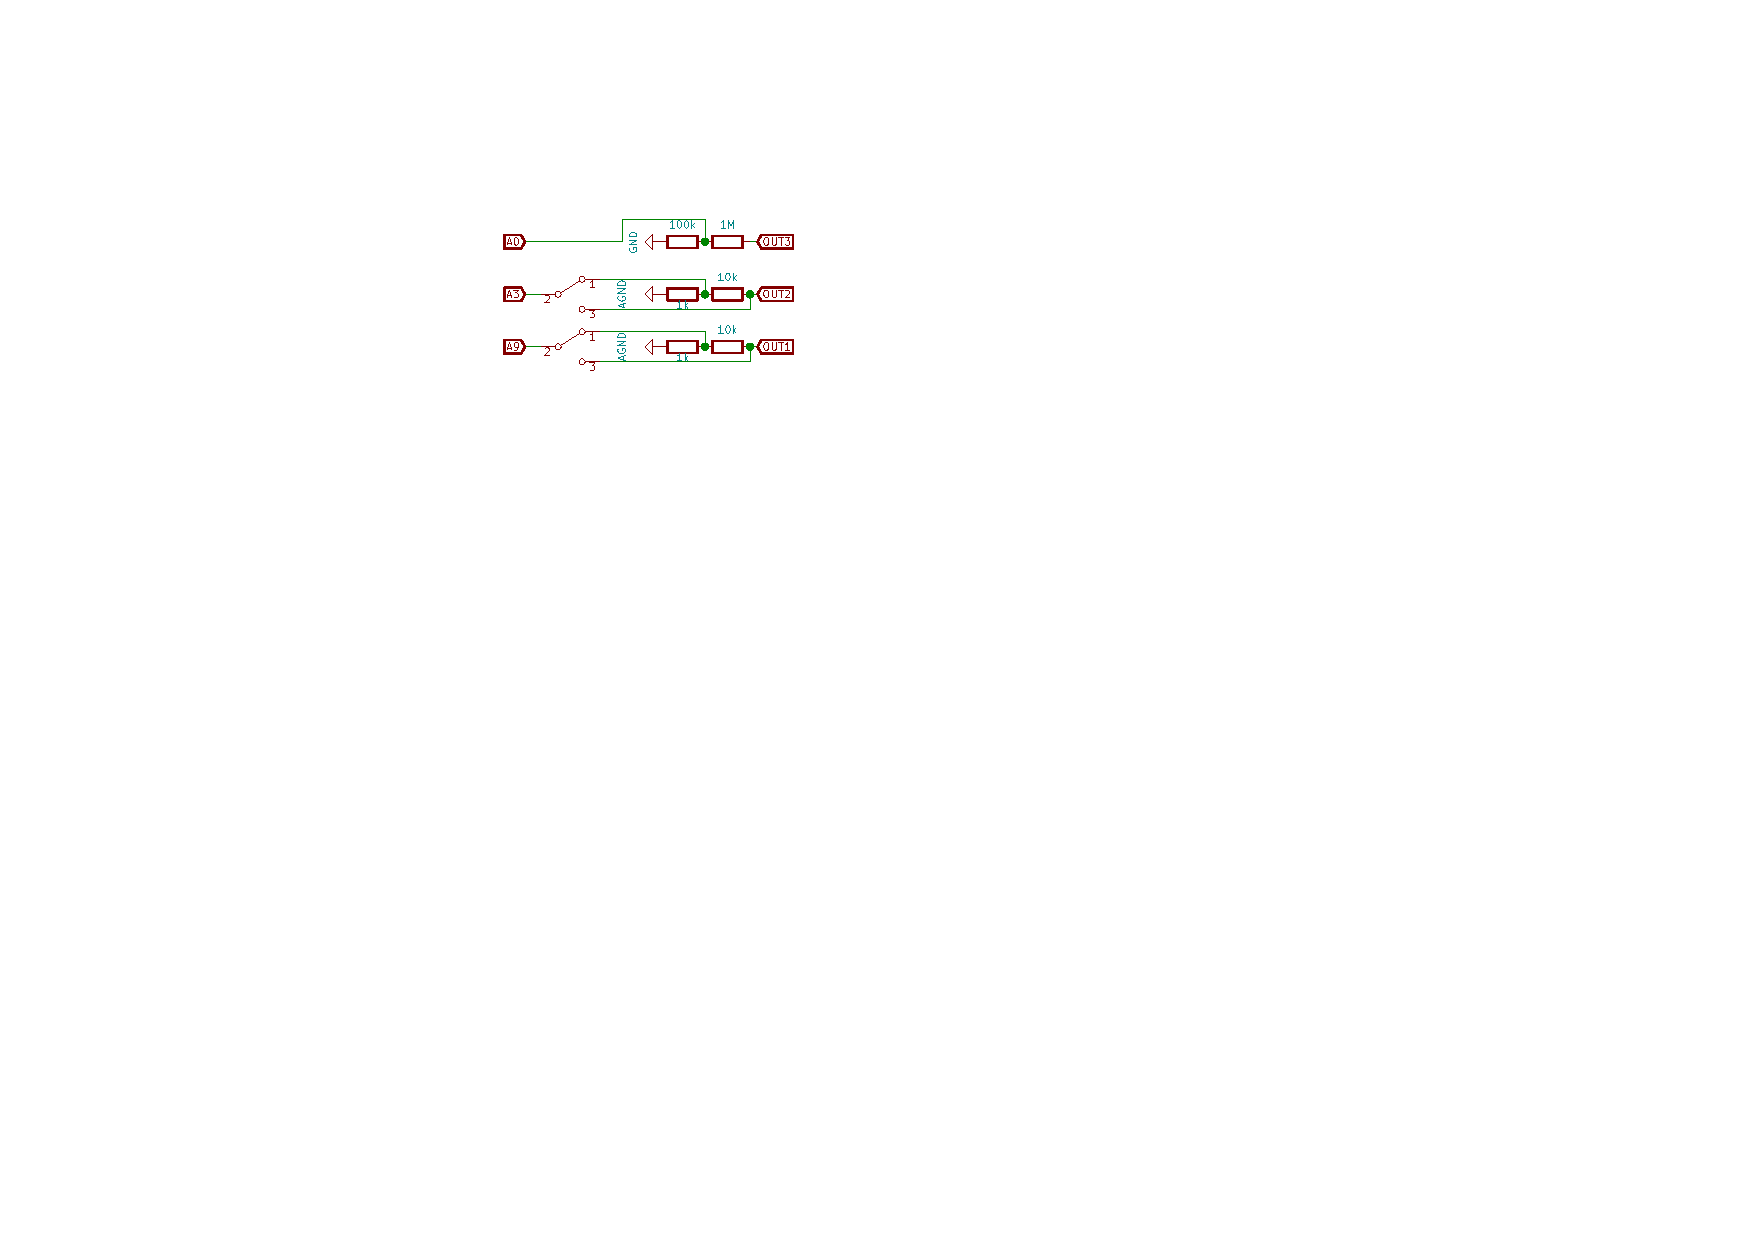
\includegraphics[scale=2.2]{./measure.pdf}
 	\caption{Schema circuitale del sistema di lettura (\texttt{Teensy})
	\label{sch:rdng}}
\end{figure}

%================================
%         Calibrazione
%================================
\subsection{Calibrazione}
I due convertitori ADC della MCU sono stati calibrati.
% continua

%================================
%       Acquisizione dati
%================================
\subsection{Acquisizione dati}
Per ogni valore scelto della resistenza R1 è stata eseguita una presa dati automatizzata secondo una routine programmata in Teensy: il condensatore viene caricato ad una tensione prefissata, una volta raggiunto il valore prestabilito viene inviato il segnale su T1, si avvia l'acquisizione sincronizzata e si attende un tempo 50 $\mu$s per permettere al MOS-FET di entrare in conduzione (R2 è stata scelta di 1k, dunque c'è un apprezzabile ritardo tra segnale e impulso) e scartare eventuali segnali spuri; a questo punto si inizia a memorizzare una serie da 100 coppie di letture -sincronizzate- ((in nota) a meno di sfasamenti nell'ordine delle centinaia di nanosecondi?), si ferma l'impulso e si trasmettono i dati al computer; se la tensione su OUT2 è stata maggiore di 3.3V si ferma l'acquisizione per non danneggiare Teensy, altrimenti si ricomincia caricando il condensatore ad una tensione più alta.

============================= OLD\newline
Vista la limitata attendibilità del circuito con interruttore azionato
manualmente si è costruito una seconda versione del circuito (Fig.
\ref{sch:gest}), in cui figurano: 
\begin{description}
	\item [Un sottocircuito] di switch	
	\item [Un condensatore] di capacità maggiore di un paio di ordini di 
	grandezza.
	\item [Teensy] La piattaforma di sviluppo impiegata per caricare
	(e scaricare) il condensatore a diverse tensioni e per la misura delle
	tensioni ai capi del diodo e della resistenza.
\end{description}

Si sviluppano due casi principali, dipendenti sostanzialmente dal valore della
resistenza $R_P$ posta in serie al diodo:\\

Se lasciamo caricare gradualmente il condensatore, essendo $C$ decisamente
maggiore rispetto ai condensatori precedenti si ha un tempo di carica
$\tau = RC$ abbastanza prolungato, in cui possiamo campionare contemporaneamente
tensione e corrente ai capi del diodo per correnti modeste, nel regime in cui
il diodo è "interdetto" ed oppone resistenza al flusso di carica.

Viceversa, nel regime in cui si applichi al diodo una d.d.p. ben al disopra di
$V_{\rm thr} \approx 0.6 $V, che siamo liberi di esplorare variando la tensione
di carica di C con il sottocircuito destro, il diodo idealmente lascia passare
tutta la corrente impressa sulla giunzione. Allora per caratterizzare la
risposta del diodo senza cambiarne drasticamente le caratteristiche (ad esempio
per eccessiva agitazione termica) si impiega il circuito di switch per
imprimere impulsi di alta corrente e breve durata sulla giunzione PN, di cui
misuriamo la curva caratteristica in risposta con i due ADC di \verb+Teensy+.

Se effettivamente il diodo, oltre ad una certa soglia di d.d.p. inizia ad avere
componente resistiva sempre più pronunciata, allora riportando le nostre
previsioni in carta semilogaritmica ci si aspetterebbe di trovare una retta,
entro il regime in cui è valida l'approssimazione di Shockley, ma oltre a
questo, una regione in cui la curva caratteristica della giunzione ora mostra
una dipendenza apprezzabilmente più lineare/ohmica dell'intensità di corrente
dalla $\Delta$V rispetto a prima, a cui corrisponderebbe il grafico "piatto"
di un logaritmo.  

%================================================================
%                   Analisi dati e Risultati
%================================================================
\section{Analisi dati e Risultati}
Il nostro intento è verificare che i dati raccolti siano in accordo con la
legge \eqref{eq: model}. Tramite la legge di Ohm è possibile ricavare la
corrente nel diodo, dividendo la caduta di tensione misurate dalla boccola
\verb'ADC0' per la resistenza $R$. Si è quindi effettuato un filtraggio volto
all'eliminazione degli outliers e dei punti meno significativi, assumendoli quali
variabili indipendenti e di natura gaussiana. Per una discussione dettagliata
del sistema di filtraggio dati si rimanda alla sezione A delle Appendici.

Successivamente, è stato effettuato un fit sulla base dei dati selezionati.
Ingenuamente, avremo dunque potuto pensare di adottare la legge 
\eqref{eq: model} direttamente. Tuttavia ciò comporterebbe il fallimento
repentino del fit a causa dei valori negativi o nulli che debitamente si
riscontrerebbero entro il logaritmo. \`E stata quindi adottata una legge
alternativa basata sul metodo delle tangenti (o di Newton). Per una trattazione
approfondita del modello di fit, si rimanda alla sezione B delle Appendici.

I dati raccolti con sovrapposta la funzione di fit sono stati posti all'interno 
del grafico \ref{fig: sck_lin}.
\begin{figure}[!htb]
	\centering 
% 		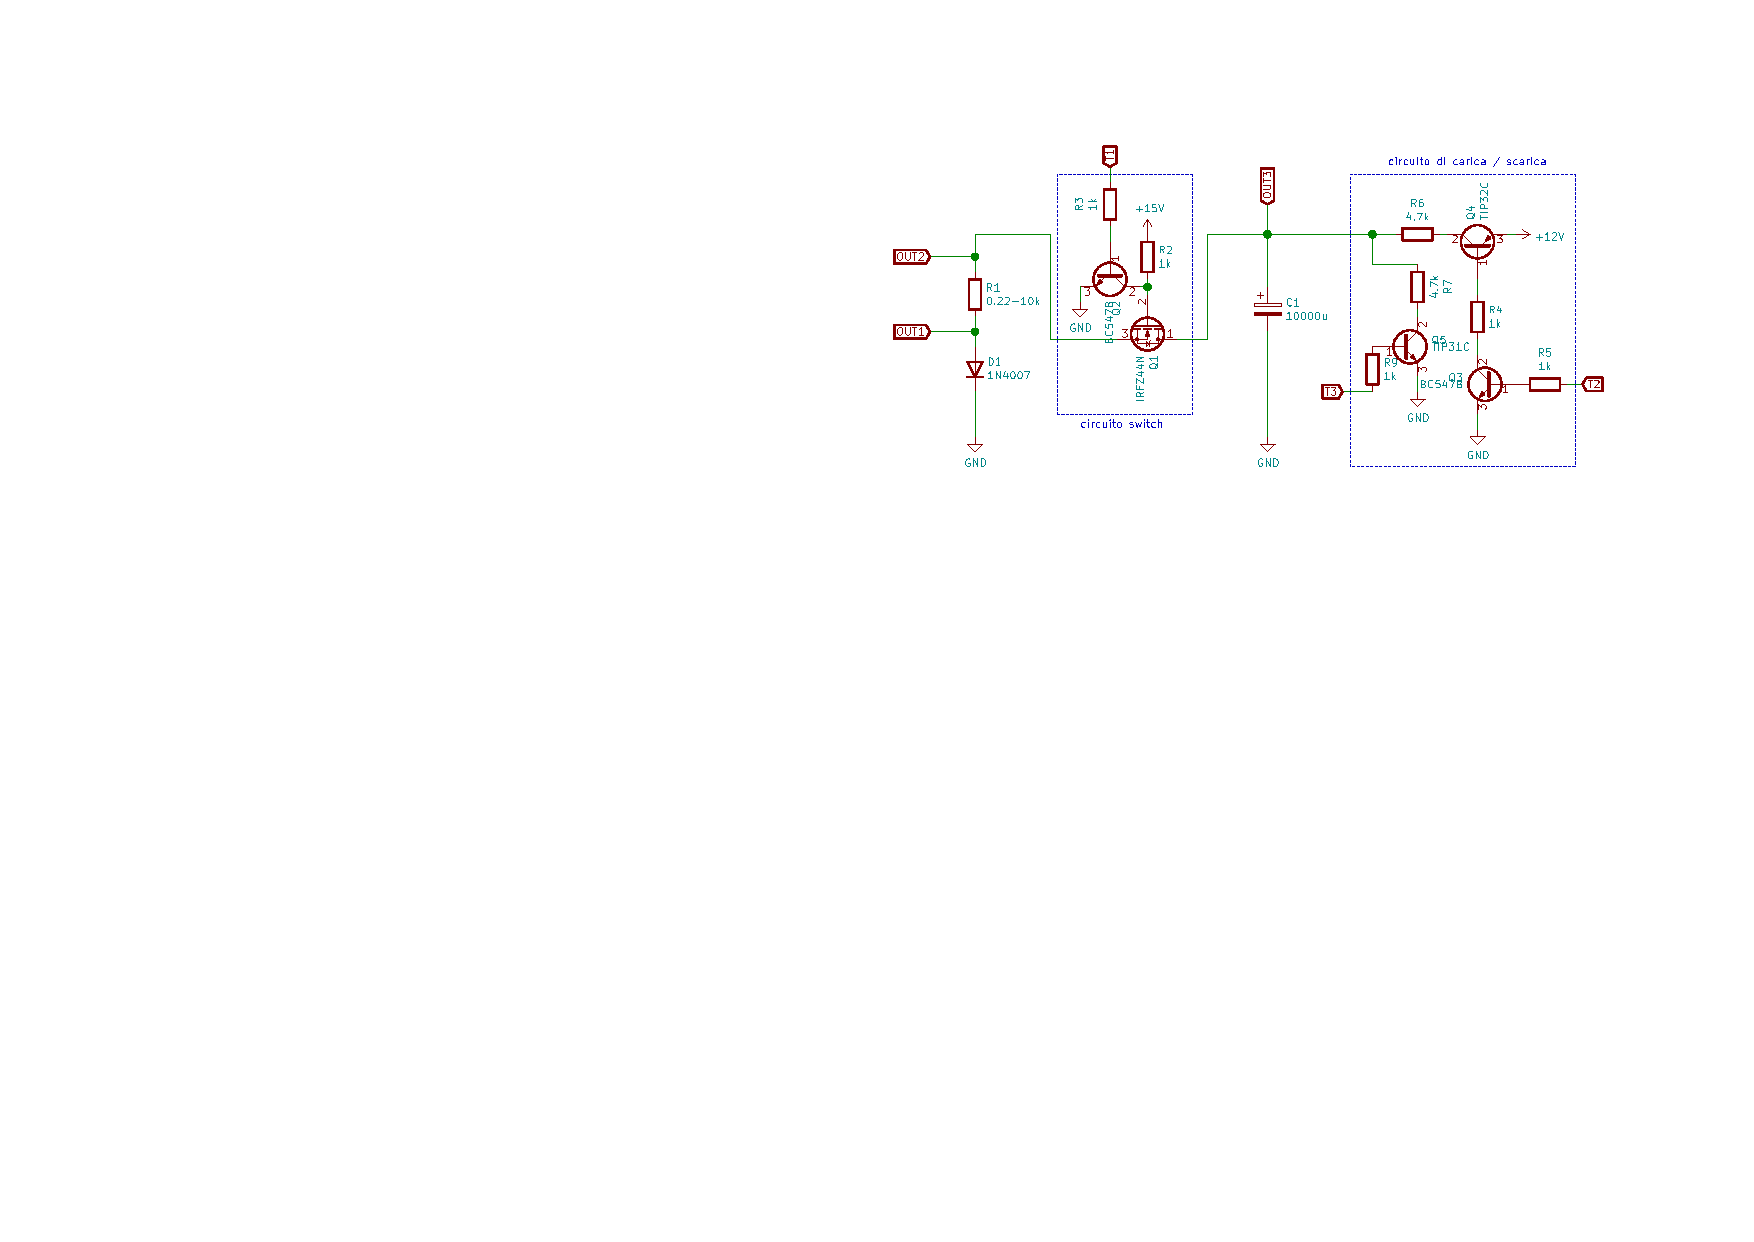
\includegraphics[scale=1.3]{./gestione.pdf}
	\caption{La curva caratteristica del diodo ricostruita dai nostri
	dati, con sovrapposto il modello di best-fit \label{fig: sck_lin}}
\end{figure}
I parametri stimati dal fit risultano essere:
\begin{align*}
	R_{diodo} &= 47.5 \pm 0.2 \; \rm m\Omega \\
	\eta V_T &= 46.40 \pm 0.06 \; \rm mV \\
	I_0 &= (3.18 \pm 0.05) \; \rm nA \\
	\sigma_{R, \eta V_T} &= ? \\   
	\sigma_{R, I_0} &= ? \\
	\sigma_{I_0, \eta V_T} &= ? \\
	\chi^2/\text{ndof} &= 4483/2760 \\
	\text{abs\_sigma} &= \rm False
\end{align*}
Il $\chi^2$ risulta essere pari a 4483 contro un aspettato di 2760.
%(i dati vanno cambiati con quelli del fit fatto bene)
Successivamente, i dati e la funzione sono stati posti all'interno di un
grafico in scala semilogaritmica (grafico \ref{fig: sck_lin}).
\begin{figure}[!htb]
	\centering 
% 		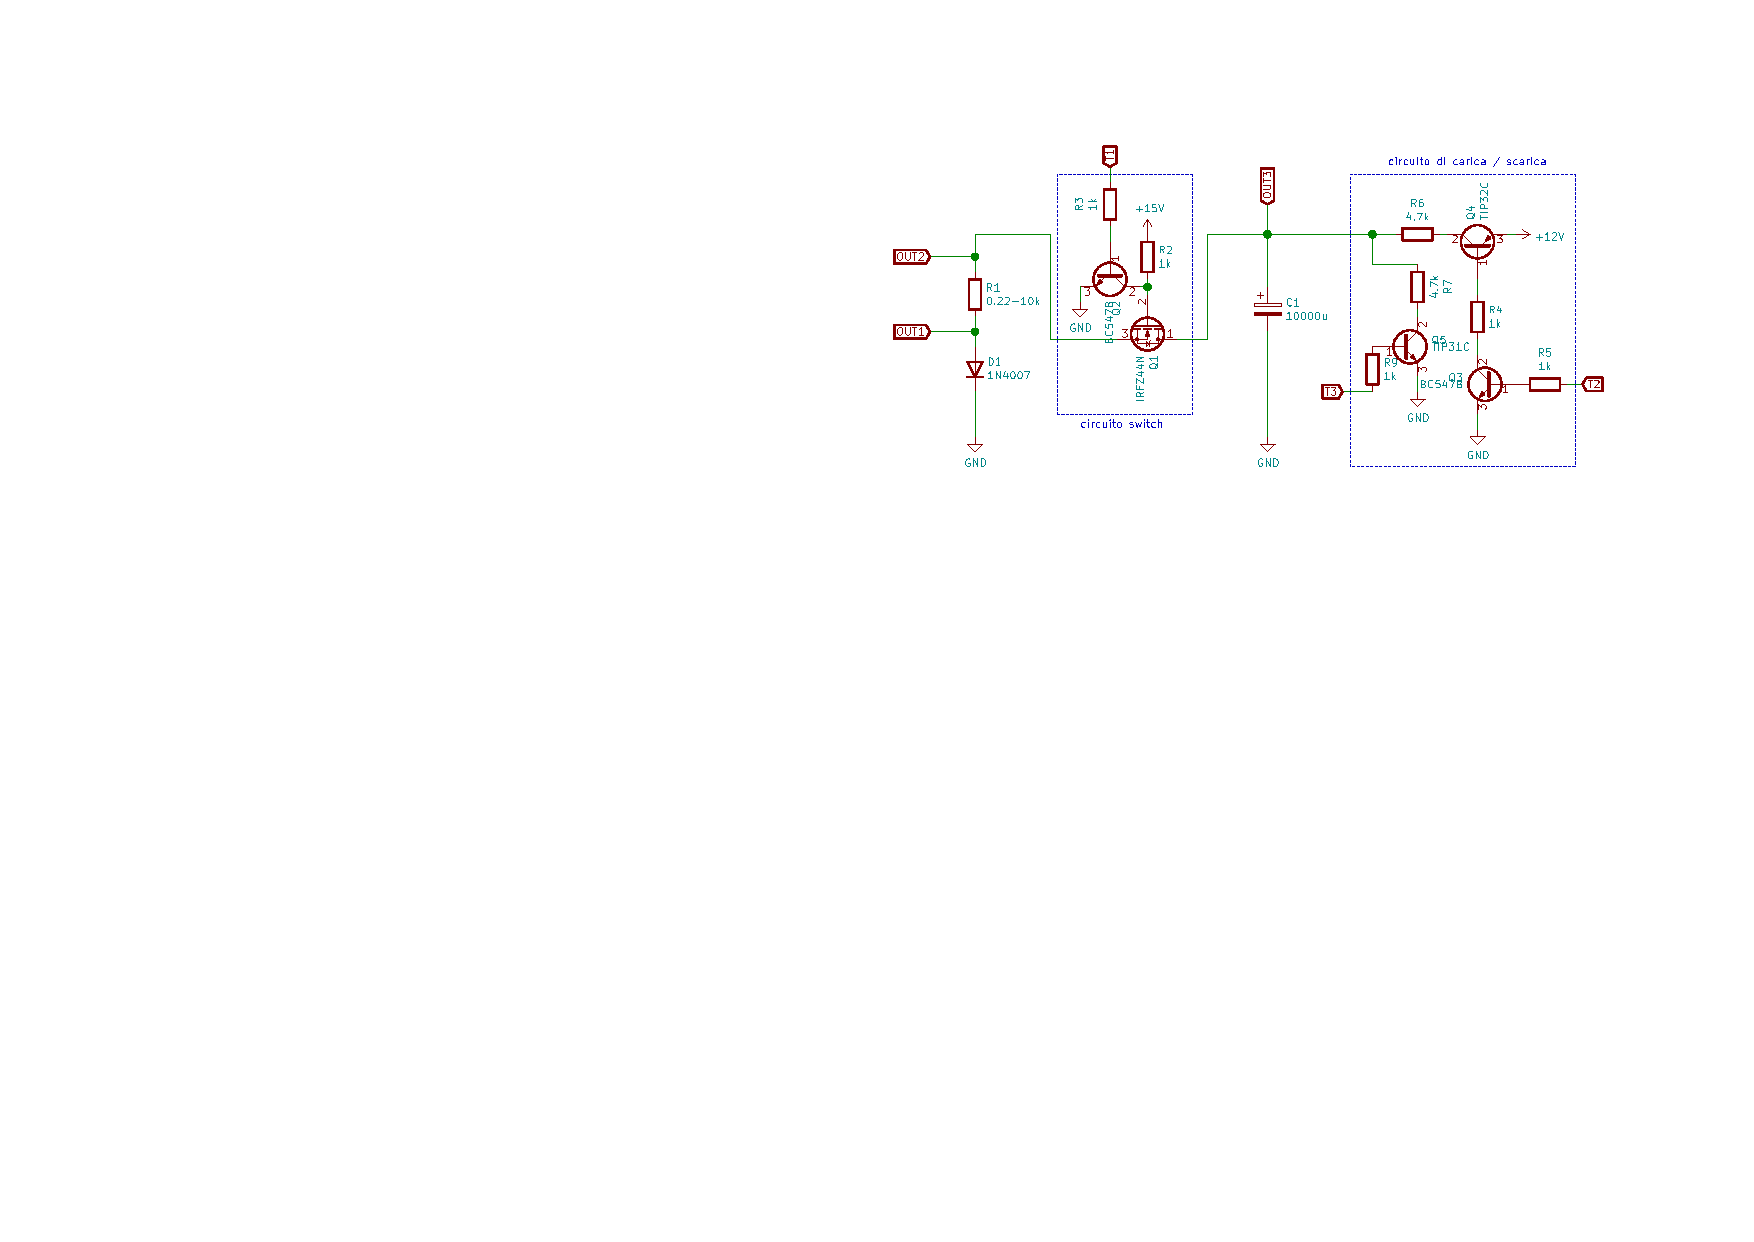
\includegraphics[scale=1.3]{./gestione.pdf}
	\caption{La stessa curva $V-I$ del diodo in scala semilogaritmica,
	con sovrapposto il modello di best-fit \label{fig: sck_log}}
\end{figure}

%================================================================
%                          Conclusioni
%================================================================
\section{Conclusioni}
L'andamento dei dati sperimentali non risulta essere ben descritto dalla legge
\eqref{eq: model}. Ciò può essere spiegato sulla base della non linearità dei
convertitori analogici digitali all'interno di Teensy 3.2, che ha comportato
degli errori difficilmente stimabili e presumibilmente correlati. Tuttavia, si
riscontrano delle analogie tra la funzione di fit ed i dati ottenuti. In
particolare, dal grafico in scala lineare, si osserva che a correnti alte
l'andamento risulta essere pressoch\`e lineare in accordo con l'ipotesi sulla
resistenza interna. Dal grafico in scala semilogaritmica, inoltre, osserviamo
che i dati risultano possedere un andamento simile a quello caratteristico 
della curva di Shockley per poi appiattirsi a partire da un particolare valore
della tensione, esattamente come ci aspetteremo da un andamento lineare.
Pertanto potremo aspettarci che i parametri stimati dal fit siano significativi.


%================================================================
%                        Appendice A
%================================================================
\section{Appendice A: Filtraggio Dati}
\subsection{Introduzione}
Durante l’esperienza si è raccolto un grande numero di dati, acquisiti in
run diversi in base alla resistenza scelta, dunque a zone differenti della
curva. Sì è posto il problema di eliminare degli outliers in modo
indipendente dal modello scelto. Inoltre le varie serie di dati si
sovrappongono, dunque è necessario eliminare quei dati che, non aggiungendo
informazioni utili, vanno a “sporcare” il grafico.

Il sistema di filtraggio di dati implementato nell'eseguibile si compone di 2
fasi: la prima è l’eliminazione di outliers, la seconda consiste
nell'eliminazione di dati non significativi.
\subsection{Procedimento}
Supponiamo di avere una serie di dati $(x, y)$ e assumiamo che siano
indipendenti tra loro. Questo non sarà in generale vero, però quest'ipotesi
è tanto più lecita quanto più la correlazione tra le varianze delle misure su
$x$ e $y$ è indipendente dai valori assunti dalle $x$ e $y$ stesse e, più
sono numerosi i dati racchiusi entro una deviazione lungo $x$: in questo caso,
infatti, la correlazione viene inclusa nella varianza lungo $y$.
Supponiamo inoltre che siano note a priori le $\sigma_x ^2 \coloneqq \var{x}$
e che la loro distribuzione di probabilità sia normale (le distribuzioni
delle componenti sono approssimativamente gaussiane per il convertitore
di Teensy, perlomeno utilizzando la risoluzione a 12 bit) secondo una matrice
di covarianza diagonale nella base $\left\{x, y\right\}$.
In ogni modo, i nostri dati $x$ e $y$ risultano indipendenti e
approssimativamente normali, dunque le assunzioni risultano giustificate. 
Allora la densità di probabilità che un punto che abbia misurato $x$ si trovi a tale ascissa
$x_i$ si ricava banalmente integrando lungo $y$ a $x$ fissata:
\[
	\ud P = \frac{1}{\sigma_{x_i} \sqrt{2\pi}}
	e^{-\frac{1}{2}{\frac{(x - x_i)^2}{\sigma_{x_i}^2}}} \ud x
.\] 
Dunque, ripetendo più volte la stessa misura, la probabilità
\[
	P\left(\mid x - x_i \mid \leq \frac{\eps}{2} \right) = \eps G_{x_i} 
.\]
dove \[
	G_{x_i} \coloneqq \frac{1}{\sigma_{x_i} \sqrt{2\pi}}
	e^{-\frac{1}{2}{\frac{(x - x_i)^2}{\sigma_{x_i}^2}}}
.\] 
e $\eps > 0$ è piccolo a piacere. Scegliendo allora solo quelle misure $x$ per
cui vale $\mid x - x_i \mid \leq \frac{\eps}{2}$, queste saranno in numero
intorno a:
\[
	N_i \coloneqq N_{\text{tot}} \frac{G_{x_i}}{\sum_j G_{x_j}} =
		N_{\text{tot}} w_i
.\] 
che definisce implicitamente i pesi $w_i$ con cui si mediano le distribuzioni
di probabilità gaussiane $G_{x_i}$.
Allora, detto:
\[
	G_{y_i} \coloneqq \frac{1}{\sigma_{y_i} \sqrt{2\pi}}
	e^{-\frac{1}{2}{\frac{(\mu_y - y_i)^2}{\sigma_{y_i}^2}}}
.\] 
Per il principio di massima verosimiglianza siamo quindi interessati a
massimizzare la quantità:
\[
	\like = \prod_{i=1}^{n} \prod_{j=1}^{N_i} G_{y_i} = 
	\prod_{i=1}^{n} G_{y_i}^{N_i}
.\] 
Per la monotonia del logaritmo il problema equivale a massimizzare la quantità:
\[
	\ln{\like} = \sum_{i=1}^{n}\ln{G_{y_i}}^{N_{\text{tot}}w_i} = 
	\frac{N_{\text{tot}}} {\sum_{j=1}^{n} G_{x_j}} 
	\sum_{i=1}^{n} G_{x_i} \ln{G_{y_i}}
.\] 
Per cui, a meno di costanti risulta:
\begin{equation}\label{eq: likeconst}
	\ln{\like} - \text{const.} \propto \sum_{i=1}^{n} -G_{x_i} \ln{\sigma_y}
	- \frac{1}{2} G_{x_i} \left( \frac{y_i - \mu_y}{\sigma_y} \right)^2
\end{equation}
Imponendo la condizione di stazionarietà rispetto a $\mu_y$ si ottiene dunque:
\begin{equation}\label{eq: muy}
	\mu_y = \sum_{i=1}^{n} y_i w_i 
\end{equation} 
Una volta sostituito in \eqref{eq: likeconst} quanto appena trovato per $\mu_y$
e imponendo la stessa condizione di stazionarietà rispetto a $\sigma_y$ si ha:
\begin{equation}\label{eq: sigmay}
	\sigma_y^2 = \sum_{i=1}^{n} (y_i - \mu_y)^2 w_i
\end{equation}
Infine è possibile ricavare la varianza di $\mu_y$ dalla definizione di valore
di aspettazione, riconducendola più volte a integrali di gaussiane di altezze
e ampiezze diverse:
\begin{align} \label{aln: varmuy}
%	\var{\mu_y} &= \sum_{i=1}^{n} w_i^2 \sigma_y^2 + 
%	\left(\frac{y_i}{\sum_{j=1}^{n} w_j}  \right)^2 \frac{
%	\frac{e^{-\frac{(x-x_i)^2}{3 \sigma_x^2}}} {\sigma_x \sqrt{6 \pi} } +
%	\frac{e^{-3\frac{(x-x_i)^2}{4 \sigma_x^2}}} {\sigma_x \sqrt{\pi} } +
%	\frac{e^{-\frac{(x-x_i)^2}{\sigma_x^2}}} {\sigma_x \sqrt{2 \pi}}
%	} {\sqrt{2 \pi}} =\\ 
	\var{\mu_y} &= \sum_{i=1}^{n} w_i^2 \sigma_y^2 + 
	\left(\frac{y_i}{\sum_{j=1}^{n} w_j} \right)^2 \frac{
	e^{-\frac{(x-x_i)^2}{3 \sigma_x^2}} +  
	\sqrt{3} \left( e^{-\frac{(x-x_i)^2}{\sigma_x^2}} -
	\sqrt{2} e^{-3 \frac{(x-x_i)^2}{4 \sigma_x^2}} \right)
	} {2 \sqrt{3}\pi \sigma_x^2} 
\end{align}
Riassumendo:\\
Nella \eqref{eq: muy} prendiamo una media dei campionamenti intorno ad un'
ascissa $x$ in esame, pesata sulla distanza che gli $x_i$ hanno da questa; 
intuitivamente lo interpretiamo come se stessimo applicando un 
\emph{blur a kernel gaussiano} ai punti acquisiti.
Effettivamente quello che stiamo facendo non è molto diverso da un stima
di densità di kernel monovariante, dove però nel nostro caso
riscaliamo la stima in base al valore assunto da $y$.
Lo stesso ragionamento vale per $\sigma_y^2$, si ha una stima della varianza
dei dati la variare di y, pesata sulla distanza dai valori studiati. Dunque
$\mu_y \pm \sigma_y$ ci dà una stima della distribuzione dei nostri dati.
\subsection{$\var{\mu_y}$}
Mentre $\sigma_y$ rappresenta la distribuzione dei dati intorno al valor medio 
$\mu_y$, $\var{\mu_y}$ ci dà un'idea dell’incertezza che attribuiamo alla
miglior stima di y. Questo ci è utile per determinare la convergenza della
stima in funzione dei dati acquisiti.
Infatti: più la densità dei dati è grande rispetto alla deviazione standard
$\sigma_x$, più la stima del valore centrale risulta precisa. Graficamente
la banda di confidenza è più ristretta dove si concentrano i dati, viceversa
tende ad allargarsi dove i dati sono sparsi, a distanze paragonabili a
$\sigma_x$. Numericamente, si vede dalla seconda somma nell'espressione
\eqref{aln: varmuy} che la stima del valore centrale è statisticamente
significativa solo quando si media su un intervallo campionato con almeno
qualche punto ogni deviazione $\sigma_x$: altrimenti $\sigma_y \to 0$
indicando assenza di dati, mentre $\var{\mu_y}$ tende a $+\infty$ come
$\sim e^{x^2}$ indice della stessa insufficienza di dati al fine di stabilire
con precisione significativa il valore di $\mu_y$.
\begin{figure}[!htb]
	\centering 
 		\includegraphics[scale=0.32]{./varmuy.pdf}
 	\caption{La media $\mu_y$ è rappresentata dalla linea rossa, mentre
	l'area in rosso indica il valore di $\var{\mu_y}$ al variare dei
	dati (in blu) lungo $x$. \label{fig: varmuy}}
\end{figure}
Nel caso opposto, in cui i dati sono "densi" (in confronto alle $\sigma_x$)
la seconda somma, per quanto computazionalmente intensiva, numericamente
sembrerebbe piccola in confronto alla prima: in realtà non lo è, ma
soprattutto questa non può essere trascurata, poiché è proprio la quantità
che descrive la dipendenza dalla densità stessa, dunque la caratteristica
convergenza/divergenza della precisione sulla stima centrale fornita.
\subsection{Filtro outliers}
La parte più semplice nel filtraggio dati consiste nello scartare tutti quei
punti che distano da $\mu_y$ più di una soglia arbitraria $k$ di deviazioni
standard $\sigma_y$ (nel nostro caso è stato scelto k = 2, non critico,
trovato dopo una serie di prove). A differenza del classico metodo basato
sulla distanza della curva modello di best fit, non siamo influenzati da
quest’ultimo. Questo risulta particolarmente utile in simili situazioni di
verifica del modello in quanto una selezione basata su un preliminare fit
risulterebbe influenzata dalla scelta della funzione in questione e
eliminerebbe tutti i dati che non risultano compatibili con essa.
%indipendentemente dal modello di fit vale $|y_i - \mu_y| \geq k\sigma_y$.
\subsection{Filtro dati non significativi}
Supponiamo di avere 2 set di dati fatti con diverse resistenze, il primo $(A)$
con una resistenza bassa, il secondo $(B)$ con una alta: Il primo set esplorerà
la regione ad alta corrente, mentre il secondo la regione di basse correnti.
In generale i dati del primo si sovrapporranno anche nelle zone basse esplorate
dal secondo, però senza aggiungere sostanziali informazioni rispetto a quanto
farebbe il secondo.
%Il nostro obiettivo è dunque eliminare questi dati meno significativi.
Esponiamo dunque il criterio sviluppato per ridurre l'influenza di questi
punti meno significativi sulla ricerca dei parametri di best-fit e sulla
rappresentazione finale dei dati.\\
Per capire se in un certo punto i dati di $A$ sono significativi, calcoliamo
la misura di significatività che abbiamo sviluppato in \eqref{aln: varmuy}$:
\var{\mu_y}$ di $A$ e di $B$. Perciò se $\var{\mu_y}$ di $A$ è maggiore di 
$q\var{\mu_y}$ di $B$, con $q$ arbitrario (nell’esperienza è stato scelto
q = 3), questo indica che i dati di $A$
ci stanno dando meno informazioni rispetto a quelli di $B$. A questo punto
è sufficiente controllare tutti i punti scorrendo su tutte le combinazioni
di set per eliminare i dati non significativi, che rendono meno
immediata l'interpretazione il grafico. Questo è ben visibile in scala
logaritmica sulle y dove i punti con grandi incertezze o varianze tendono
a disperdersi rapidamente.
L’algoritmo è computazionalmente intensivo e richiede una corretta gestione
della memoria per evitare bolle di allocazione, dunque è stato implementato
in C++ per praticità e richiamato all’interno degli script.
Nelle figure di esempio sono mostrati i dati selezionati dall’algoritmo
(in nero) ed i dati scartati (in rosso). 
E’ infine mostrato il confronto dei grafici delle $\var(\mu_y)$
tra due set successivi.

\begin{figure}[!htb]
	\centering 
 		\includegraphics[scale=0.9]{./nofilter.pdf}
	\caption{Grafico in scala semilogaritmica prima del filtraggio dati:
	si evidenziano in rosso i dati da scartare, in nero quello tenuti.
	\label{fig: nofilter}}
\end{figure}
\begin{figure}[!htb]
	\centering 
 		\includegraphics[scale=0.9]{./filtered.pdf}
 	\caption{Grafico in scala semilogaritmica dopo il filtraggio dati.
	\label{fig: filtered}}
\end{figure}
\begin{figure}[!htb]
	\centering 
 		\includegraphics[scale=0.32]{./comparison.pdf}
 	\caption{Confronto dei grafici delle $\var{\mu_y}$ su due set di
	dati consecutivi. \label{fig: comparison}}
\end{figure}

%================================================================
%                        Appendice b
%================================================================
\section{Appendice B: Metodo di Fit}
Partiamo dall'osservazione che la tensione ai capi del diodo può essere
scomposta in $\Delta V_r$ e $\Delta V_d$ come illustrato in figura:
\begin{center}
\begin{circuitikz}
\draw (-2, 0)
	to[dcvsource, v=$\Delta V$, *-] (0,0)
	to[R=$r$, v=$\Delta V_r$, *-*] (2,0)
	to[Do, v=$\Delta V_d$,  *-*] (5,0)
	node[ground]{};
\draw[gray, dashed] (-2,-2)--(-2,2)--(5,2)--(5,-2)--cycle;
\end{circuitikz}
\end{center}
dove il resistore a sinistra indica proprio la resistenza di un diodo reale,
mentre il diodo alla sua destra rappresenta una giunzione bipolare PN, ossia
il diodo ideale descritto dall’equazione di Shockley.
Dunque ci aspettiamo che la tensione $V$ campionata con \verb+Teensy+ ai capi
del diodo rispetti la legge:
\begin{equation}\label{eq: invsck}
V = \Delta V = \Delta V_d + \Delta V_r = \eta V_T = \ln{\frac{I+I_0}{I_0}} + RI
\end{equation}
All’interno dello script \verb'fit_file.py', voltages rappresenta il vettore
delle ascisse dei punti campionati, mentre currents rappresenta l'analogo per
le ordinate. Le incertezze associate a questi due all'interno dello script
prendono i nomi \verb'voltageErrs' e \verb'currentErrs'.
Ingenuamente potremmo essere tentati di effettuare una sorta di fit “inverso”
(delle x in funzione delle y).
Tuttavia una tale operazione non è affatto banale, a causa dei valori 
negativi/nulli che debitamente si riscontreranno all’interno del logaritmo
nella legge \eqref{eq: invsck}, che possono facilmente portare al fallimento
dell'algoritmo di fit.
\`E per questo che si è dovuto definire il modello "inverso" nella forma di
una legge di natura approssimata per ricorsione, grazie al metodo di Newton. 
Al livello di implementazione si è quindi dichiarata una funzione:
\begin{lstlisting}[label={lst: curr}]
def curr(V, I0, nVt, R):
    v = V
    for i in range(Nstep):
	a = deriv_errFun(v, I0, nVt, R)
	v = v - errFun(v, V, I0, nVt, R) /a
    return (V - v)/R
\end{lstlisting}

Questa verrà in seguito usata come modello per la corrente in funzione della
tensione ai capi del diodo reale nella routine di fit per minimi quadrati.
La funzione \verb'curr' cerca di -linearizzare- la relazione tra $I$ e $V$
nell'intorno di un determinato $V$. Come sappiamo infatti dal metodo di Newton:
detta $f(x)$ una funzione tale che $f(x) = 0$ e, dato un valore iniziale
tale che $f(x[0]) = \alpha$ generico, sappiamo che la relazione di ricorsione
\begin{align}
	x[0] = \alpha \\ \label{aln: newton}
	x[N+1] = x[N] - \frac{f(x[N])}{f'(x[N])}
\end{align}
converge ad un valore approssimato per la nostra $x$, commettendo un errore 
sempre più piccolo al crescere di $N$, indice del livello di ricorsione
raggiunto. 
Nel nostro caso $x$ sarà quella tensione $v$ per cui vale l'identità:
\begin{equation}\label{eq: sck}
	I(V) \coloneqq I_0^{\frac{\Delta V}{\eta V_T}} = \frac{V - v}{R}	
\end{equation}
che identifica il tratto lineare descritto da una retta con coefficiente
angolare negativo pari a $-\frac{1}{R}$ ed intercetta $I = v/R$ 
sull’asse delle ordinate; si tratta proprio della retta di carico del diodo.
L'equazione ricorsiva \eqref{aln: newton} ci permette quindi di determinare
il punto di lavoro $v$ per cui la corrente (di lavoro) si può scrivere come
$\frac{V - v}{R}$, come si vede dal return nella funzione di fit
\verb'curr(V, parametri liberi)'.
A questo punto si può già intuire quali siano le altre due funzioni di
appoggio richiamate dentro \verb'curr', di cui riportiamo le definizioni
per completezza:
\begin{lstlisting}[label={lst: errFun}]
def sck(V, I0, nVt):
    return I0*(pylab.exp(V/nVt) - 1)

def errFun(V, V0, I0, nVt, R):
    return sck(V, I0, nVt) + (V - V0)/R

def deriv_errFun(V, I0, nVt, R):
    return I0 / nVt * pylab.exp(V/nVt) + 1./R
\end{lstlisting}
Infatti \verb'errFun' e \verb'deriv_errFun' sono, rispettivamente, la relazione 
da minimizzare specificata dalla legge \eqref{eq: sck} e la sua derivata
rispetto a $V$.
In conclusione, si è effettuato un fit dei minimi quadrati implementato in
\verb+Python+ mediante la funzione \emph{curve\_fit} dal modulo \verb+optimize+
interno alla libreria \texttt{Scipy}\cite{scipy} adottando come modello
\verb'curr' e lasciando liberi tutti i suoi parametri.
In particolare si è tenuto conto dell'incertezza sulla variabile indipendente
con il metodo "dell'errore efficace": ovvero propagando gli errori 
\verb'voltageErrs' sulle $V$, tramite le stime dei parametri ottenute da un fit
preliminare, in cui prendiamo \verb'currentErrs' come sole incertezze sulla
variabile dipendente $I$. Lo stesso algoritmo di fit viene iterato più volte,
però assumendo come incertezza sulle misure una sorta di errore efficace 
dato dalla somma in quadratura dei due contributi all'incertezza: 
\begin{equation}\label{eq: seff}
	\Delta_{\text{eff}_i} \coloneqq \sqrt{\left|\frac{\ud \, curr}{\ud V}
	\right|_{V = V_i} \Delta_{V_i}^2 + \Delta_{I_i}^2}.
\end{equation}
fin a che non converge ai valori ottimali dei parametri.
\medskip
\bibliographystyle{IEEEtrandoi}
\bibliography{refs}
\end{document}
